\documentclass{article}
    \usepackage{url}
    \usepackage{cite}    
    \usepackage{xcolor}
    \usepackage{lscape}
    \usepackage{amssymb}
    \usepackage{titling}
    \usepackage{pdfpages}
    \usepackage{enumitem}
    \usepackage{graphicx}
    \usepackage{hyperref}
    \usepackage{listings}
    \usepackage{fancybox}
    \usepackage{enumerate}
    \usepackage{pdflscape}
    \usepackage{afterpage}
    \usepackage{lstautogobble}
    \usepackage[margin=0.8in]{geometry}
    \usepackage[nottoc,notlot,notlof]{tocbibind}
    \renewcommand\maketitlehookd{\vfill\null}
    \renewcommand\maketitlehooka{\null\mbox{}\vfill}

    \newcommand\backgroundimage{
        \put(-5,0){
        \parbox[b][\paperheight]{\paperwidth}{
        \vfill
        \centering
        \includegraphics[height=\paperheight]{\graphicspath{background.jpg}}
        \vfill
    }}}

    \newcounter{num}

    \graphicspath{ {Images/} }

    \title{EBUS3030 Assignment 1}
    \author{
        Steven Karmaniolos 
        \texttt{c3160280@uon.edu.au}\\
        Jay Rovacsek
        \texttt{c3146220@uon.edu.au}\\
        Jacob Litherland
        \texttt{c3263482@uon.edu.au}\\
        Edward Lonsdale
        \texttt{c3252144@uon.edu.au}
    }
    \date{\today}
    \hypersetup{
    colorlinks=true,
    linkcolor=black,
    filecolor=magenta,      
    urlcolor=blue,
    citecolor=red,
    linktoc=section,
    }
    \pagenumbering{arabic}

    \newlist{legal}{enumerate}{10}
    \setlist[legal]{label*=\arabic*.}

    \begin{document}

    \begin{titlingpage}
        \maketitle
    \end{titlingpage}

    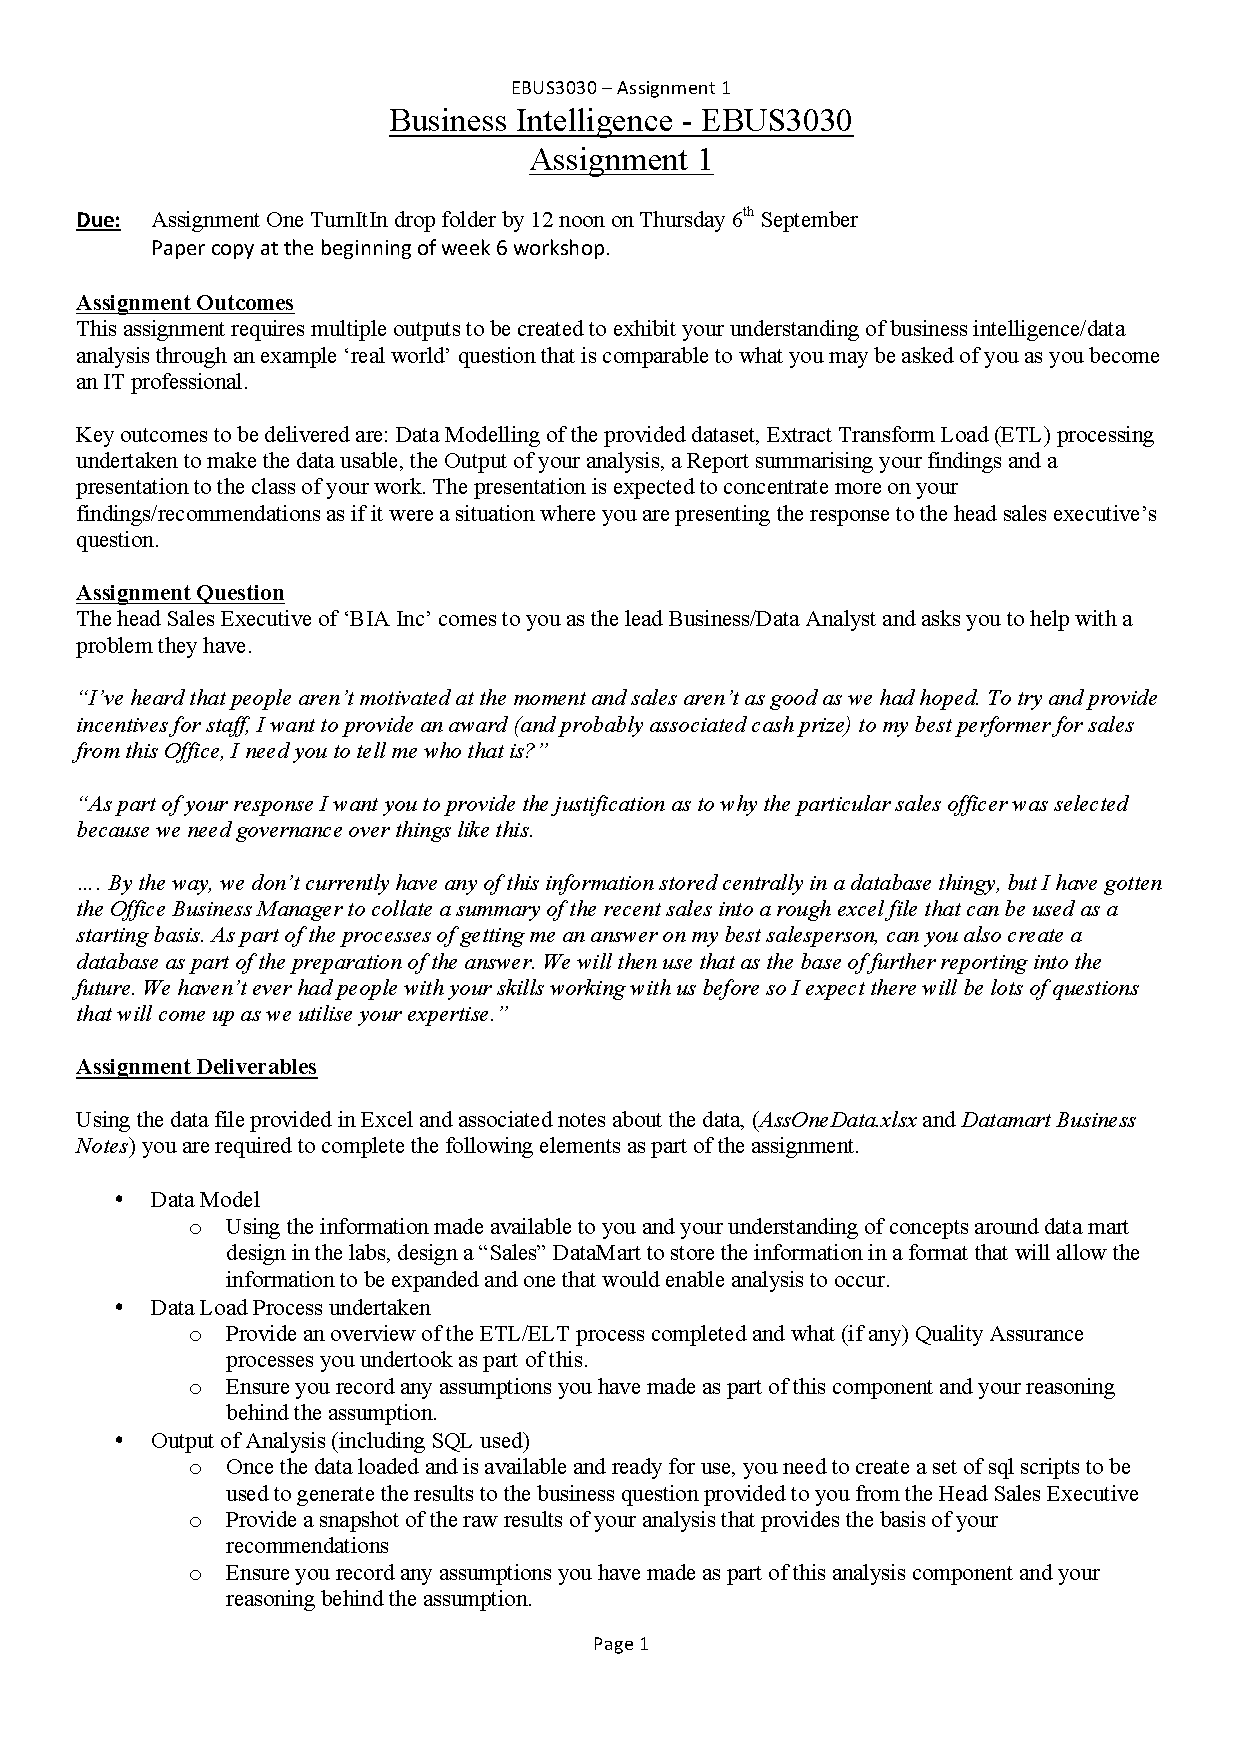
\includepdf[height=\paperheight,keepaspectratio,pages={1,2}]{Resources/Assignment1Overview.pdf}

    \section{Datamart Business Notes}
    The following business rules were provided to be used in the context of this assignment:
    \begin{itemize}
        \renewcommand\labelitemi{*}
        \item At BIA all customers interacts are in an online environment, 
        there are no orders outside of electronic.
        \item Returning customers can provide POI information via the web
        interface and look up their record and that will flow with the sale.
        \item The sales associate can complete the order form/sale for the
        client.
        \item Each sale will have a reciept number/id.
        \item A reciept can have many line items.
        \item Each line item can only be for a single item, but the customer can
        purchase multiples of the same item.
        \item Where a customer has multiple line items, any sale with more than
        5 row items (containing at least 5 different items) is provided a
        15\% discount.
        \item The system automatically handles the total for the sale by looking
        up the item, then multiplying the costs per item by number
        purchased, and then should store this final field total as a record
        in the system (but should also be able to see clearly sales that
        were provided a discount.
        \item Item prices can change at any point, and the price the customer
        pays is the amount listed for the item on the sale date. We need to
        keep a record of all item prices historically.
        \item Only 1 BIA sales assistant can be attributed to any receipt.
    \end{itemize}

    \newpage
    \section{Data Model}

    \newpage
    \section{Data Load Process (ETL/ELT)}
        \subsection{Quality Assurance Processes}
        \subsection{Assumptions and Reasoning}

    \newpage
    \section{Base Analysis}
        \subsection{Raw Results}

    \newpage
    \section{Executive Summary}

    \newpage
    \section{Assumptions}

    \newpage
    \begin{thebibliography}{9}
        \raggedright
        \bibitem{Placeholder}
            Placeholder
            \url{www.placeholder.com}
    \end{thebibliography}

    \newpage
    \section{Appendix}
    \label{sec:Appendix}

    \end{document}
